\documentclass[11pt]{article}

\usepackage{fontspec}
\usepackage{polyglossia}
\usepackage{amsmath}
\usepackage{amssymb}
\usepackage{xcolor}
\usepackage{fancyhdr}
\usepackage{graphicx}
\usepackage{listings}
\usepackage[most]{tcolorbox}
% \usepackage{setspace}
\usepackage{pifont}
\usepackage{enumitem}
\usepackage{titlesec}
\usepackage[bottom]{footmisc}
\usepackage{titling}
\usepackage{minted}
\usepackage{etoolbox}
\usepackage{array}
\usepackage{extsizes}
\usepackage{float}
\usepackage{booktabs}
\usepackage{hyperref}
\usepackage[onehalfspacing]{setspace}
\usepackage[a4paper, top=2.7cm, bottom=2.7cm, left=2.5cm, right=2.5cm, headheight=1.5cm, headsep=0.5cm]{geometry}
\usepackage{tikz}

\usetikzlibrary{automata, positioning, arrows.meta, arrows}

\newfontfamily\emoji{Segoe UI Emoji}

\pagestyle{fancy}

\setmainlanguage[numerals=western]{arabic}
\setotherlanguage{english}
% \newfontfamily\arabicfont[Script=Arabic]{Amiri}
\newfontfamily\arabicfont[Script=Arabic]{Calibri}
\newfontfamily\arabicfonttt[Script=Arabic]{Courier New}

\lstset{
  language=[Sharp]C,
  numbers=left,
  stepnumber=1,
  numbersep=8pt,
  frame=single,
  basicstyle=\ttfamily\small,
  keywordstyle=\color{blue},
  stringstyle=\color{red},
  commentstyle=\color{green!50!black}
}

\newif\ifdetailed
\ifdefined\setdetailed
  \setdetailed
\fi

\newif\ifwithsols
\ifdefined\setwithsols
  \setwithsols
\fi

% unified tcolorboxes for articles
\tcbset{colback=white, colframe=black, fonttitle=\bfseries, boxrule=0.8pt}
\newtcolorbox{boxDef}[1][]{colback=blue!5!white,colframe=blue!75!black,
  title={{\emoji📘} تعريف\ifx\\#1\\\else ~#1\fi :}}
\newtcolorbox{boxExercise}[1][]{colback=cyan!5!white,colframe=cyan!70!black,
  title={{\emoji🧩} تمرين\ifx\\#1\\\else ~#1\fi :}}
\newtcolorbox{boxExample}[1][]{colback=yellow!5!white,colframe=orange!90!black,
  title={{\emoji📝} مثال\ifx\\#1\\\else ~#1\fi :}}
\newtcolorbox{boxNote}[1][]{colback=gray!10!white,colframe=black,
  title={{\emoji✨} ملاحظة\ifx\\#1\\\else ~#1\fi :}}
\newtcolorbox{boxAttention}[1][]{colback=magenta!10!white,colframe=magenta!80!black,
  title={{\emoji🔔} تنبيه\ifx\\#1\\\else ~#1\fi :}}
\newtcolorbox{boxWarning}[1][]{colback=red!5!white,colframe=red!75!black,
  title={{\emoji⚡} ملاحظة هامة\ifx\\#1\\\else ~#1\fi :}}
\newtcolorbox{boxSolution}[1][]{colback=green!5!white,colframe=green!60!black,
  title={{\emoji✅} حل\ifx\\#1\\\else ~#1\fi :}}
\newtcolorbox{boxSymbol}[1][]{colback=purple!5!white,colframe=purple!70!black,
  title={{\emoji🔣} رمز\ifx\\#1\\\else ~#1\fi :}}
\newtcolorbox{boxHint}[1][]{colback=teal!5!white,colframe=teal!60!black,
  title={{\emoji💡} تلميح\ifx\\#1\\\else ~#1\fi :}}


\tcbset{simplecode/.style={ colback=gray!5, colframe=black!50, boxrule=0.4pt, arc=2pt, left=4pt,right=4pt,top=4pt,bottom=4pt}}
\newenvironment{boxCode}{\begin{tcolorbox}[simplecode]}{\end{tcolorbox}}

\newcolumntype{C}[1]{>{\centering\arraybackslash}p{#1}}

% redefine spaces after titles
\makeatletter
\renewcommand{\@maketitle}{%
  \begin{center}
    {\huge \bfseries \@title \par}%
    \vskip 0.2em % space between title and author
    {\large \@author \par}%
    % \vskip 0.2em % space between author and date
    % {\normalsize \@date \par}%
  \end{center}
}
\makeatother

\fancyhf{} % clear default
\fancypagestyle{plain}{
  \fancyhf{}
  \fancyhead[L]{مدرسة التسامح الشاملة}
  % \fancyhead[L]{
\includegraphics[height=1cm]{../../../images/logoTasamoh.png}}
  \fancyhead[R]{الأستاذ محمود اغبارية}
  \fancyfoot[C]{\thepage}
}

\fancyhead[L]{مدرسة التسامح الشاملة}
\fancyhead[R]{الأستاذ محمود اغبارية}
\fancyfoot[C]{\thepage}
% \date{\today}

\setcounter{tocdepth}{3} % only section subsection and subsubsection in TOC

\newcommand{\importpdfpage}[2]{%
    \thispagestyle{empty}
    \newgeometry{left=0cm,right=0cm,top=0cm,bottom=0cm}
    \includegraphics[page=#2,width=0.95\paperwidth,height=0.95\paperheight,keepaspectratio]{#1}
    \restoregeometry
}

\newcommand{\insertFullImg}[1]{%
    \noindent
    \makebox[\textwidth][c]{
        \includegraphics[width=0.9\paperwidth,keepaspectratio]{#1}%
    }%
}%

% ----------------------


% \begin{document}

% \maketitle

% % \clearpage  % start TOC on a new page
% % \renewcommand{\contentsname}{جدول المحتويات}
% % \tableofcontents
% % \clearpage

% \part*{part 1} % the * prevents numbering
% \section*{مقدمة}
% \subsection*{مثال رياضي}
% \subsubsection*{مثال فرعي}
% \paragraph*{ paragraph 1}
% \subparagraph*{sub paragraph 1}

% \ifdetailed
% \begin{english}
% \begin{minted}{csharp}
% // C# Example
% \end{minted}
% \end{english}
% \fi

% OLD WAY
% \ifdetailed
% \begin{english}
% \begin{lstlisting}
% // C# Example
% \end{lstlisting}
% \end{english}
% \fi

% % 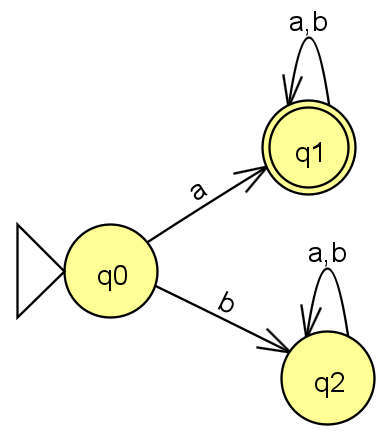
\includegraphics[width=0.2\textwidth]{../../../images/DFAs/ex1_q1.png}



% \vspace{3cm}
% \begin{flushleft}
% أرجو لكم وقتًا ممتعًا.

% الأستاذ محمود اغبارية.
% \end{flushleft}


% \end{document}


\title{أمثلة شاملة: الفئات والكائنات في \textenglish{C\#}}

\begin{document}
\maketitle
\thispagestyle{fancy}

\section*{الخطوة 1 - تعريف الفئة وإنشاء كائن}
\begin{boxExample}[الخطوة 1 - تعريف الفئة وإنشاء كائن]
\begin{english}
\begin{minted}{csharp}
class Book
{
    public string Title;
    public string Author;
    public int Year;
    public double Price;
}
internal class Program
{
    public static void Main(string[] args)
    {
        Book b = new Book();
        b.Title = "Algebra";
        b.Author = "Teacher";
        b.Year = 2020;
        b.Price = 100.0;

        Book b2 = new Book();
        b2.Title = "Geometry";
        b2.Author = "Teacher";
        b2.Year = 2022;
        b2.Price = 150.0;
    }
}
\end{minted}
\end{english}
\end{boxExample}

\clearpage
\section*{الخطوة 2 - العمليات الداخلية بدون معاملات}
\begin{boxExample}[الخطوة 2 - العمليات الداخلية بدون معاملات]
\begin{english}
\begin{minted}{csharp}
class Book
{
    public string Title;
    public string Author;
    public int Year;
    public double Price;

    public void Print()
    {
        Console.WriteLine($"{Author}: {Title} ({Year})");
    }
}
internal class Program
{
    public static void PrintBook(Book b)
    {
        Console.WriteLine($"{b.Author}: {b.Title} ({b.Year})");
    }
    public static void Main(string[] args)
    {
        Book b1 = new Book();
        b1.Title = "Algebra";
        b1.Author = "Teacher";
        b1.Year = 2020;
        b1.Price = 100.0;
        b1.Print();

        Book b2 = new Book();
        b2.Title = "Geometry";
        b2.Author = "Teacher";
        b2.Year = 2022;
        b2.Price = 150.0;
        PrintBook(b2);
    }
}
\end{minted}
\end{english}
\end{boxExample}

\clearpage
\section*{الخطوة 3 - العمليات الداخلية بمعاملات}
\begin{boxExample}[الخطوة 3 - العمليات الداخلية بمعاملات]
\begin{english}
\begin{minted}{csharp}
class Book
{
    public string Title;
    public string Author;
    public int Year;
    public double Price;

    public void Print()
    {
        Console.WriteLine($"{Author}: {Title} ({Year})");
    }

    public bool WasPublishedBefore(int year)
    {
        return Year < year;
    }
}
\end{minted}
\end{english}
\end{boxExample}
\begin{boxExample}[تتمة - الخطوة 3 - العمليات الداخلية بمعاملات]
\begin{english}
\begin{minted}{csharp}
internal class Program
{
    public static void Main(string[] args)
    {
        Book b1 = new Book();
        b1.Title = "Algebra";
        b1.Author = "Teacher";
        b1.Year = 2020;
        b1.Price = 100.0;
        b1.Print();
        if(b1.WasPublishedBefore(2021))
            Console.WriteLine("The book was published before 2021.");

        Book b2 = new Book();
        b2.Title = "Geometry";
        b2.Author = "Teacher";
        b2.Year = 2022;
        b2.Price = 150.0;
        b2.Print();
        if (b2.WasPublishedBefore(2021))
            Console.WriteLine("The book was published before 2021.");
        else
            Console.WriteLine("The book was published in 2021 or later.");
    }
}
\end{minted}
\end{english}
\end{boxExample}

\clearpage
\section*{الخطوة 3.1 - مقارنة كائنين: \textenglish{IsEqualTo} مقابل \textenglish{==}}
\begin{boxExample}[الخطوة 3.1 - مقارنة كائنين: \textenglish{IsEqualTo} مقابل \textenglish{==}]
\begin{english}
\begin{minted}{csharp}
class Book
{
    public string Title;
    public string Author;
    public int Year;
    public double Price;

    public void Print()
    {
        Console.WriteLine($"{Author}: {Title} ({Year})");
    }

    public bool WasPublishedBefore(int year)
    {
        return Year < year;
    }

    public bool IsEqualTo(Book other)
    {
        return Title == other.Title
            && Author == other.Author
            && Year == other.Year;
    }
}
\end{minted}
\end{english}
\end{boxExample}
\begin{boxExample}[تتمة - الخطوة 3 - العمليات الداخلية بمعاملات]
\begin{english}
\begin{minted}{csharp}
internal class Program
{
    public static void Main(string[] args)
    {
        Book b1 = new Book();
        b1.Title = "Algebra";
        b1.Author = "Teacher";
        b1.Year = 2020;
        b1.Price = 100.0;

        Book b2 = new Book();
        b2.Title = "Algebra";
        b2.Author = "Teacher";
        b2.Year = 2020;
        b2.Price = 100.0;

        if (b1 == b2)
            Console.WriteLine("b1 == b2");
        else
            Console.WriteLine("b1 != b2");

        if(b1.IsEqualTo(b2))
            Console.WriteLine("b1 is equal to b2");
        else
            Console.WriteLine("b1 is not equal to b2");
    }
}
\end{minted}
\end{english}
\end{boxExample}

\clearpage
\section*{الخطوة 3.2 - الكلمة المفتاحية \textenglish{this}}
\begin{boxExample}[الخطوة 3.2 - الكلمة المفتاحية \textenglish{this}]
\begin{english}
\begin{minted}{csharp}
class Book
{
    public string Title;
    public string Author;
    public int Year;
    public double Price;

    public void Print()
    {
        Console.WriteLine($"{Author}: {Title} ({Year})");
    }

    public bool WasPublishedBefore(int year)
    {
        return Year < year;
    }

    public bool IsEqualTo(Book other)
    {
        return this.Title == other.Title
            && this.Author == other.Author
            && this.Year == other.Year;
    }
}
\end{minted}
\end{english}
\end{boxExample}
\begin{boxExample}[تتمة - الخطوة 3 - العمليات الداخلية بمعاملات]
\begin{english}
\begin{minted}{csharp}
internal class Program
{
    public static void Main(string[] args)
    {
        Book b1 = new Book();
        b1.Title = "Algebra";
        b1.Author = "Teacher";
        b1.Year = 2020;
        b1.Price = 100.0;

        Book b2 = new Book();
        b2.Title = "Algebra";
        b2.Author = "Teacher";
        b2.Year = 2020;
        b2.Price = 100.0;

        if (b1 == b2)
            Console.WriteLine("b1 == b2");
        else
            Console.WriteLine("b1 != b2");

        if(b1.IsEqualTo(b2))
            Console.WriteLine("b1 is equal to b2");
        else
            Console.WriteLine("b1 is not equal to b2");
    }
}
\end{minted}
\end{english}
\end{boxExample}

\clearpage
\section*{الخطوة 3.3 - القيمة \textenglish{null} والتحقق منها}
\begin{boxExample}[الخطوة 3.3 - القيمة \textenglish{null} والتحقق منها]
\begin{english}
\begin{minted}{csharp}
class Book
{
    public string Title;
    public string Author;
    public int Year;
    public double Price;

    public void Print()
    {
        Console.WriteLine($"{Author}: {Title} ({Year})");
    }

    public bool WasPublishedBefore(int year)
    {
        return Year < year;
    }

    public bool IsEqualTo(Book other)
    {
        if(other == null)
            return false;

        return this.Title == other.Title
            && this.Author == other.Author
            && this.Year == other.Year;
    }
}
\end{minted}
\end{english}
\end{boxExample}
\begin{boxExample}[تتمة - الخطوة 3 - العمليات الداخلية بمعاملات]
\begin{english}
\begin{minted}{csharp}
internal class Program
{
    public static void Main(string[] args)
    {
        Book b1 = new Book();
        b1.Title = "Algebra";
        b1.Author = "Teacher";
        b1.Year = 2020;
        b1.Price = 100.0;

        Book b2 = new Book();
        b2.Title = "Algebra";
        b2.Author = "Teacher";
        b2.Year = 2020;
        b2.Price = 100.0;

        Book b3 = null;

        if(b1.IsEqualTo(b3))
            Console.WriteLine("b1 is equal to b3");
        else
            Console.WriteLine("b1 is not equal to b3");
    }
}
\end{minted}
\end{english}
\end{boxExample}

\clearpage
\section*{الخطوة 4 - العملية البنّاءة (\textenglish{Constructor})}
\begin{boxExample}[الخطوة 4 - العملية البنّاءة (\textenglish{Constructor})]
\begin{english}
\begin{minted}{csharp}
class Book
{
    public string Title;
    public string Author;
    public int Year;
    public double Price;

    public Book(string title, string author, int year, double price)
    {
        this.Title = title;
        this.Author = author;
        this.Year = year;
        this.Price = price;
    }

    public void Print()
    {
        Console.WriteLine($"{Author}: {Title} ({Year})");
    }

    public bool WasPublishedBefore(int year)
    {
        return Year < year;
    }

    public bool IsEqualTo(Book other)
    {
        if (other == null)
            return false;

        return this.Title == other.Title
            && this.Author == other.Author
            && this.Year == other.Year;
    }
}
\end{minted}
\end{english}
\end{boxExample}
\begin{boxExample}[تتمة - الخطوة 4 - العملية البنّاءة (\textenglish{Constructor})]
\begin{english}
\begin{minted}{csharp}
internal class Program
{
    public static void Main(string[] args)
    {
        Book b1 = new Book("Algebra", "Teacher", 2020, 100.0);
        Book b2 = new Book("Geometry", "Teacher", 2022, 150.0);
        b1.Print();
    }
}
\end{minted}
\end{english}
\end{boxExample}

\clearpage
\section*{الخطوة 5.1 - عمليات الاسترجاع (\textenglish{Getters})}
\begin{boxExample}[الخطوة 5.1 - عمليات الاسترجاع (\textenglish{Getters})]
\begin{english}
\begin{minted}{csharp}
class Book
{
    private string Title;
    private string Author;
    private int Year;
    private double Price;

    public Book(string title, string author, int year, double price)
    {
        this.Title = title;
        this.Author = author;
        this.Year = year;
        this.Price = price;
    }

    public string GetTitle()
    {
        return Title;
    }
    public string GetAuthor()
    {
        return Author;
    }

    public int GetYear()
    {
        return Year;
    }

    public double GetPrice()
    {
        return Price;
    }

\end{minted}
\end{english}
\end{boxExample}
\begin{boxExample}[تتمة - الخطوة 5.1 - عمليات الاسترجاع (\textenglish{Getters})]
\begin{english}
\begin{minted}{csharp}
    public void Print()
    {
        Console.WriteLine($"{Author}: {Title} ({Year})");
    }

    public bool WasPublishedBefore(int year)
    {
        return Year < year;
    }

    public bool IsEqualTo(Book other)
    {
        if (other == null)
            return false;

        return this.Title == other.Title
            && this.Author == other.Author
            && this.Year == other.Year;
    }
}
internal class Program
{
    public static void Main(string[] args)
    {
        Book b1 = new Book("Algebra", "Teacher", 2020, 100.0);
        Book b2 = new Book("Geometry", "Teacher", 2022, 150.0);
        b1.Print();
        Console.WriteLine(b2.GetTitle());
        Console.WriteLine(b2.GetAuthor());
        Console.WriteLine(b2.Author); // ERROR
    }
}
\end{minted}
\end{english}
\end{boxExample}

\clearpage
\section*{الخطوة 5.2 - عمليات التعديل (\textenglish{Setters})}
\begin{boxExample}[الخطوة 5.2 - عمليات التعديل (\textenglish{Setters})]
\begin{english}
\begin{minted}{csharp}
class Book
{
    private string Title;
    private string Author;
    private int Year;
    private double Price;

    public Book(string title, string author, int year, double price)
    {
        this.Title = title;
        this.Author = author;
        this.Year = year;
        this.Price = price;
    }

    public string GetTitle()
    {
        return Title;
    }
    public string GetAuthor()
    {
        return Author;
    }

    public int GetYear()
    {
        return Year;
    }

    public double GetPrice()
    {
        return Price;
    }

\end{minted}
\end{english}
\end{boxExample}
\begin{boxExample}[تتمة - الخطوة 5.2 - عمليات التعديل (\textenglish{Setters})]
\begin{english}
\begin{minted}{csharp}
    public void SetPrice(double newPrice)
    {
        if(newPrice > 0)
            Price = newPrice;
    }

    public void Print()
    {
        Console.WriteLine($"{Author}: {Title} ({Year})");
    }

    public bool WasPublishedBefore(int year)
    {
        return Year < year;
    }

    public bool IsEqualTo(Book other)
    {
        if (other == null)
            return false;

        return this.Title == other.Title
            && this.Author == other.Author
            && this.Year == other.Year;
    }
}
internal class Program
{
    public static void Main(string[] args)
    {
        Book b1 = new Book("Algebra", "Teacher", 2020, 100.0);
        Book b2 = new Book("Geometry", "Teacher", 2022, 150.0);
        Console.WriteLine(b2.GetPrice()); // 150.0
        b2.SetPrice(120.0);
        Console.WriteLine(b2.GetPrice()); // 120.0
        b2.SetPrice(-100); // will do nothing
        Console.WriteLine(b2.GetPrice()); // 120.0
    }
}
\end{minted}
\end{english}
\end{boxExample}


\section*{الخطوة 6 - عمليات داخلية إضافية}
\begin{boxExample}[الخطوة 6 - عمليات داخلية إضافية]
\begin{english}
\begin{minted}{csharp}
class Book
{
    private string Title;
    private string Author;
    private int Year;
    private double Price;

    public Book(string title, string author, int year, double price)
    {
        this.Title = title;
        this.Author = author;
        this.Year = year;
        this.Price = price;
    }

    public string GetTitle()
    {
        return Title;
    }
    public string GetAuthor()
    {
        return Author;
    }

    public int GetYear()
    {
        return Year;
    }

    public double GetPrice()
    {
        return Price;
    }

    public void SetPrice(double newPrice)
    {
        if(newPrice > 0)
            Price = newPrice;
    }
\end{minted}
\end{english}
\end{boxExample}
\begin{boxExample}[تتمة - الخطوة 6 - عمليات داخلية إضافية]
\begin{english}
\begin{minted}{csharp}
    public void Print()
    {
        Console.WriteLine($"{Author}: {Title} ({Year})");
    }

    public bool WasPublishedBefore(int year)
    {
        return Year < year;
    }

    public bool IsEqualTo(Book other)
    {
        if (other == null)
            return false;

        return this.Title == other.Title
            && this.Author == other.Author
            && this.Year == other.Year;
    }

    public void ApplyDiscount(int ratio)
    {
        this.Price = this.Price * (100 - ratio) / 100;
    }
}
internal class Program
{
    public static void Main(string[] args)
    {
        Book b1 = new Book("Algebra", "Teacher", 2020, 100.0);
        Console.WriteLine(b1.GetPrice()); // 100.0
        b1.ApplyDiscount(20);
        Console.WriteLine(b1.GetPrice()); // 80.0
    }
}
\end{minted}
\end{english}
\end{boxExample}

\end{document}
